\section{Methodology}

Building on the work of \citet{altae2017low}, we implement a Random Forest and a GCN as benchmark models. Additionally, we implement four few-shot machine learning architectures: Siamese Networks, Matching Networks, Prototypical Networks, and Relation Networks. IterRefLSTMs \citep{altae2017low}, used in the state-of-the-art, are used to enrich the resulting embeddings in latent space. Molecules are represented as graph objects and subsequently processed using GCNs to produce a vectorised embedding in computational space. We try to follow the implementation of \citet{altae2017low} as closely as possible for reproducibility and homogenising of results for effective comparison.

\subsection{Machine Learning Pipeline}

The machine learning pipeline for this study consists of nine main parts, which are illustrated in Figure~\ref{fig:architecture-schematic} and described hereunder:

\begin{enumerate}
    \item \textbf{Data Acquisition}. We utilise three main publicly available datasets for this study, namely, Tox21, MUV, and the GPCR subset of DUD-E. The latter is a new contribution to the study by \citet{altae2017low}. All data is available as SMILES strings with a flag for the experimental assays in the dataset recording whether the molecule is active or an inactive/decoy.

    \item \textbf{Standardise molecule}. The SMILES strings are first standardised to transform all molecular representations according to a set of well-defined and consistent rules and conventions to ensure validity and uniformity.

    \item \textbf{Molecular features generation}. The molecular graph generated from the standardised SMILES representation is enriched with atom descriptors to add information to the molecular representation.

    \item \textbf{Molecular graphs generation}. The molecular representations are transformed into graph objects, consisting of nodes and edges representing atoms and bonds, respectively. The connectivity between atoms is represented via an adjacency matrix.

    \item \textbf{Episode generation}. Effective few-shot learning necessitates that conditions at training match those at testing \citep{vinyals2016matching}. Therefore, $N$-way $K$-shot support sets and queries are randomly sampled to form a series of episodes for training. $K$ in each support set is constrained between one and ten examples per class. For every episode, we have two classes, the active class and the inactive/decoy class.

    \item \textbf{Learning a molecular embedding}. The sampled molecules in each episode are used to learn a molecular embedding using GCNs.

    \item \textbf{Few-Shot Learning}. The learned embeddings are processed using four different meta-learning architectures: Siamese, Matching, Prototypical and Relation Networks. IterRefLSTMs \citep{altae2017low} are used to enrich the model. A subset of experimental assays in each dataset is reserved for training, while the rest are reserved for testing.

    \item \textbf{Testing}. The trained models are subsequently used to test on new experimental assays, previously unseen during training, to gauge the generalising capability of a model trained for a low-data scenario. Support sets are randomly sampled and trained on the remaining molecules in the dataset for 20 rounds. The mean and standard deviation of the areas under the curve for Precision-Recall (PR-AUC) and Receiver Operator Characteristic (ROC-AUC) are calculated to quantify performance.

    \item \textbf{Evaluation}. Finally, we evaluate the results based on the ROC-AUC and PR-AUC scores from the 20 test rounds. We apply statistical analysis for results obtained across different experiments to determine the best-performing techniques for each support set composition. Confusion matrices, ROC-AUC and PR-AUC graphs for the experiment with the median ROC-AUC score from the 20 rounds are generated after test completion.
\end{enumerate}

\begin{figure}[!ht]
    \centering
    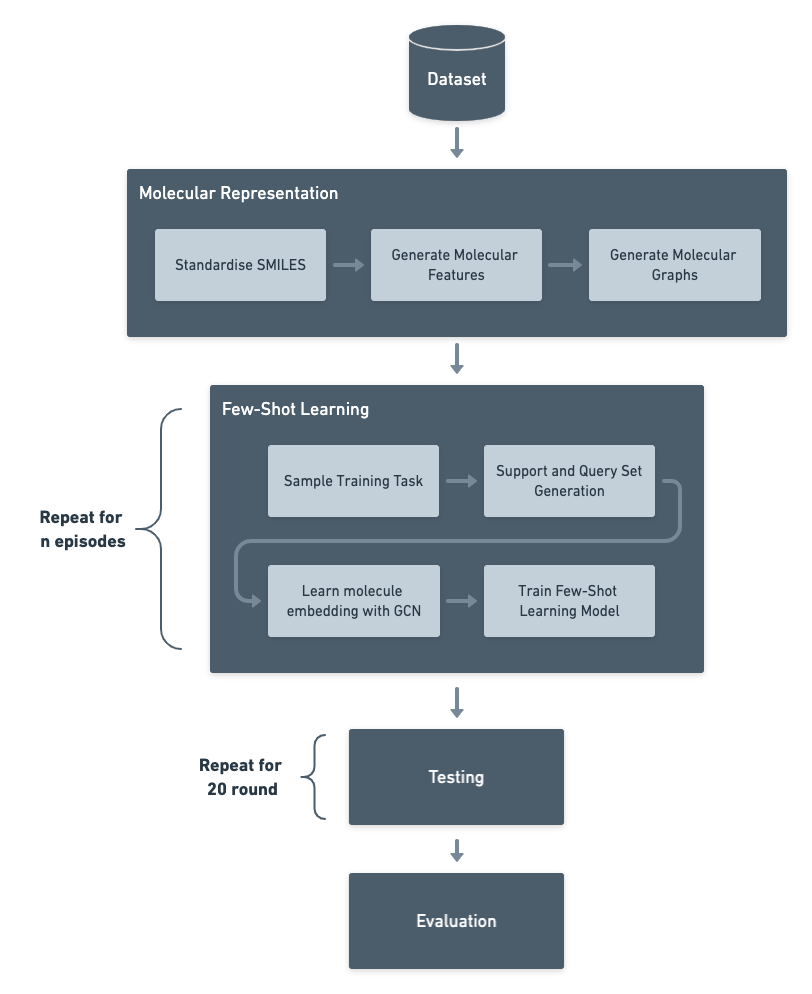
\includegraphics[width=0.9\linewidth]{img/architecture-schematic.png}
    \caption[Schematic of the major parts in our architecture]{Schematic of the machine learning pipeline designed for this study. The changes across few-shot learning architectures lie in the `Train Few-Shot Learning Model' component. Otherwise, all other modules remain identical. Figure \ref{fig:schematiconeshotdrug} visualises the GCN learned embedding as \textit{g}' and \textit{f}', and the few-shot learning steps as \textit{g, f, k}.}
    \label{fig:architecture-schematic}
\end{figure}

\subsection{Datasets}

In this work, we make use of the following three datasets;

\begin{itemize}
    
    \item \textbf{Tox21} \citep{huang2016tox21challenge} -- Mainly used for lead optimisation, containing toxicity data for 12 targets \citep{tox21}. The dataset was obtained from the DeepChem AWS bucket\footnote{Accessed from: \url{https://deepchemdata.s3-us-west-1.amazonaws.com/datasets/tox21.csv.gz}. Last Accessed: 26/05/2022} in CSV format. The NR-AR, NR-AR-LBD, NR-AhR, NR-Aromatase, NR-ER, NR-ER-LBD, NR-PPAR-gamma, SR-ARE, SR-ATAD5 targets are reserved for training, and the remaining SR-HSE, SR-MMP, SR-p53 targets are used for testing.
    
    \item \textbf{Maximum Unbiased Validation (MUV)} \citep{rohrer2009maximum} -- Based on PubChem BioAssays, used for validating virtual screening techniques against 17 different targets \citep{rohrer2009maximum}. The dataset was obtained from the DeepChem AWS bucket\footnote{Accessed from: \url{https://deepchemdata.s3-us-west-1.amazonaws.com/datasets/muv.csv.gz}. Last Accessed: 26/05/2022} in CSV format. A total of 12 targets (MUV-466, MUV-548, MUV-600, MUV-644, MUV-652, MUV-689, MUV-692, MUV-712, MUV-713, MUV-733, MUV-737, and MUV-810) are reserved for training, while MUV-832, MUV-846, MUV-852, MUV-858, and MUV-859 are reserved for testing.
    
    \item \textbf{Directory of Useful Decoys (Enhanced) (DUD-E)} \cite{mysinger2012directory} -- Used for benchmarking virtual screening techniques by introducing active compounds against specific targets. Many \textit{decoys} with similar physical properties but different topologies are made available for each active molecule. We used the GPCR subset of the DUD-E dataset \citep{mysinger2012directory} for this research study. The data was obtained directly from the DUD-E website.\footnote{Accessed from: \url{http://dude.docking.org/subsets/gpcr}. Last Accessed: 26/05/2022} The AA2AR, DRD3, and ADRB1 targets are used for training. Two targets, ADRB2 and CXCR4, are reserved for testing. We note that this is an additional contribution to the study from \citet{altae2017low}.
\end{itemize}

Table~\ref{table:datasetimbalance} shows the excessive imbalance of these datasets, highlighting the scarceness of data on active compounds in this domain. Due to this class imbalance, we also report PR-AUC metrics in addition to the ROC-AUC metrics presented in the study by \citet{altae2017low}.

\begin{table}[h]
    \centering
    \caption{Number of actives and inactives/decoys across all targets in the datasets used. Figures in parentheses show the percentage of the total compounds in the dataset.}
    \begin{tabular}{@{}crr@{}}
        \hline
        Dataset         & Actives           & Inactives/Decoys \\
        \hline
        Tox21           & 4,149 (7.04\%)    & 54,746 (92.96\%) \\
        MUV             & 347 (0.20\%)      & 175,990 (99.80\%) \\
        DUD-E (GPCR)    & 1,249 (1.45\%)    & 84,856 (98.55\%) \\
        \hline              
    \end{tabular}
    \label{table:datasetimbalance}
\end{table}

\subsection{Molecular Representations}

We first standardise the molecules according to well-defined and consistent rules and conventions. Maintaining uniformity and integrity across the different data is of utmost importance. \citet{bento2020open} present an open source chemical structure curation pipeline based on RDKit\citep{rdkit} for validating and standardising chemical structures, which follow FDA/IUPAC guidelines \citep{brecher2006graphical, food2007substance}. Their work is available in the ChEMBL Structure Pipeline package \citep{bento2020open} and is used to standardise the molecules in our pipeline. 

We create a molecular graph from the SMILES string of the standardised molecule using RDKit, an open-source toolkit for cheminformatics. We then one-hot encode eight atom features in each molecule: atom type, atomic number, atom degree, explicit valence, hybridisation, formal charge, number of radical electrons, and aromaticity. Self-loops are added to every node in the generated graph, so aggregation functions during message passing consider the features of the node itself. The order of the atoms follows the canonical order of the atoms assigned through RDKit. We make use of the Deep Graph Library (DGL) LifeSci \cite{dgllife} library to create the graph objects and subsequently process them using the DGL library \cite{wang2019dgl}.

\subsection{Episodic Learning}

Training for few-shot learning is carried out in a series of episodes, as shown in Figure \ref{fig:architecture-schematic}. We consider $N$-way $K$-shot classification tasks for each episode, where the support set contains \textit{N} classes and \textit{K} labelled molecules. The tasks in our research are binary classification tasks. Therefore \textit{N} is always set to two to represent the active and the inactive/decoy class, respectively. Experiments with varying values of \textit{K} are carried out to generate the support sets, with a minimum of one data point, to a maximum of ten data points (molecules) per class. The combinations for \textit{K} active and inactive/decoy classes are not exhaustive, but we follow the support set composition used in \citet{altae2017low} to compare results with this study directly.

Table~\ref{table:support-set-sizes} contains the composition of the support sets used in our experiments. For each episode, we sample a total of 128 query molecules composed of a balanced combination of molecules from each class. If the active class for a specific target contains less than 64 molecules, the active molecules are over-sampled such that each query set contains 64 actives. The choice of the support set composition was based on the methodology presented in \citet{altae2017low}.

\begin{table}
    \centering
    \begin{tabular}{@{}rrr@{}}
        \hline
        Actives & Inactives/Decoys & Support Set Size \\
        \hline
        10  & 10 & 20 \\
        5   & 10 & 15 \\
        1   & 10 & 11 \\
        1   & 5  & 6 \\
        1   & 1  & 2 \\
        \hline
    \end{tabular}
    \caption{Support set composition}
    \label{table:support-set-sizes}
\end{table}

\subsection{Machine Learning Models}

Before processing the molecular graph, the model first learns an embedding using GCNs. Four different architectures, including Siamese, Matching, Prototypical and Relation Networks, subsequently process the learned graph embeddings to train our meta-learner.

\begin{figure}[ht!]
    \centering
    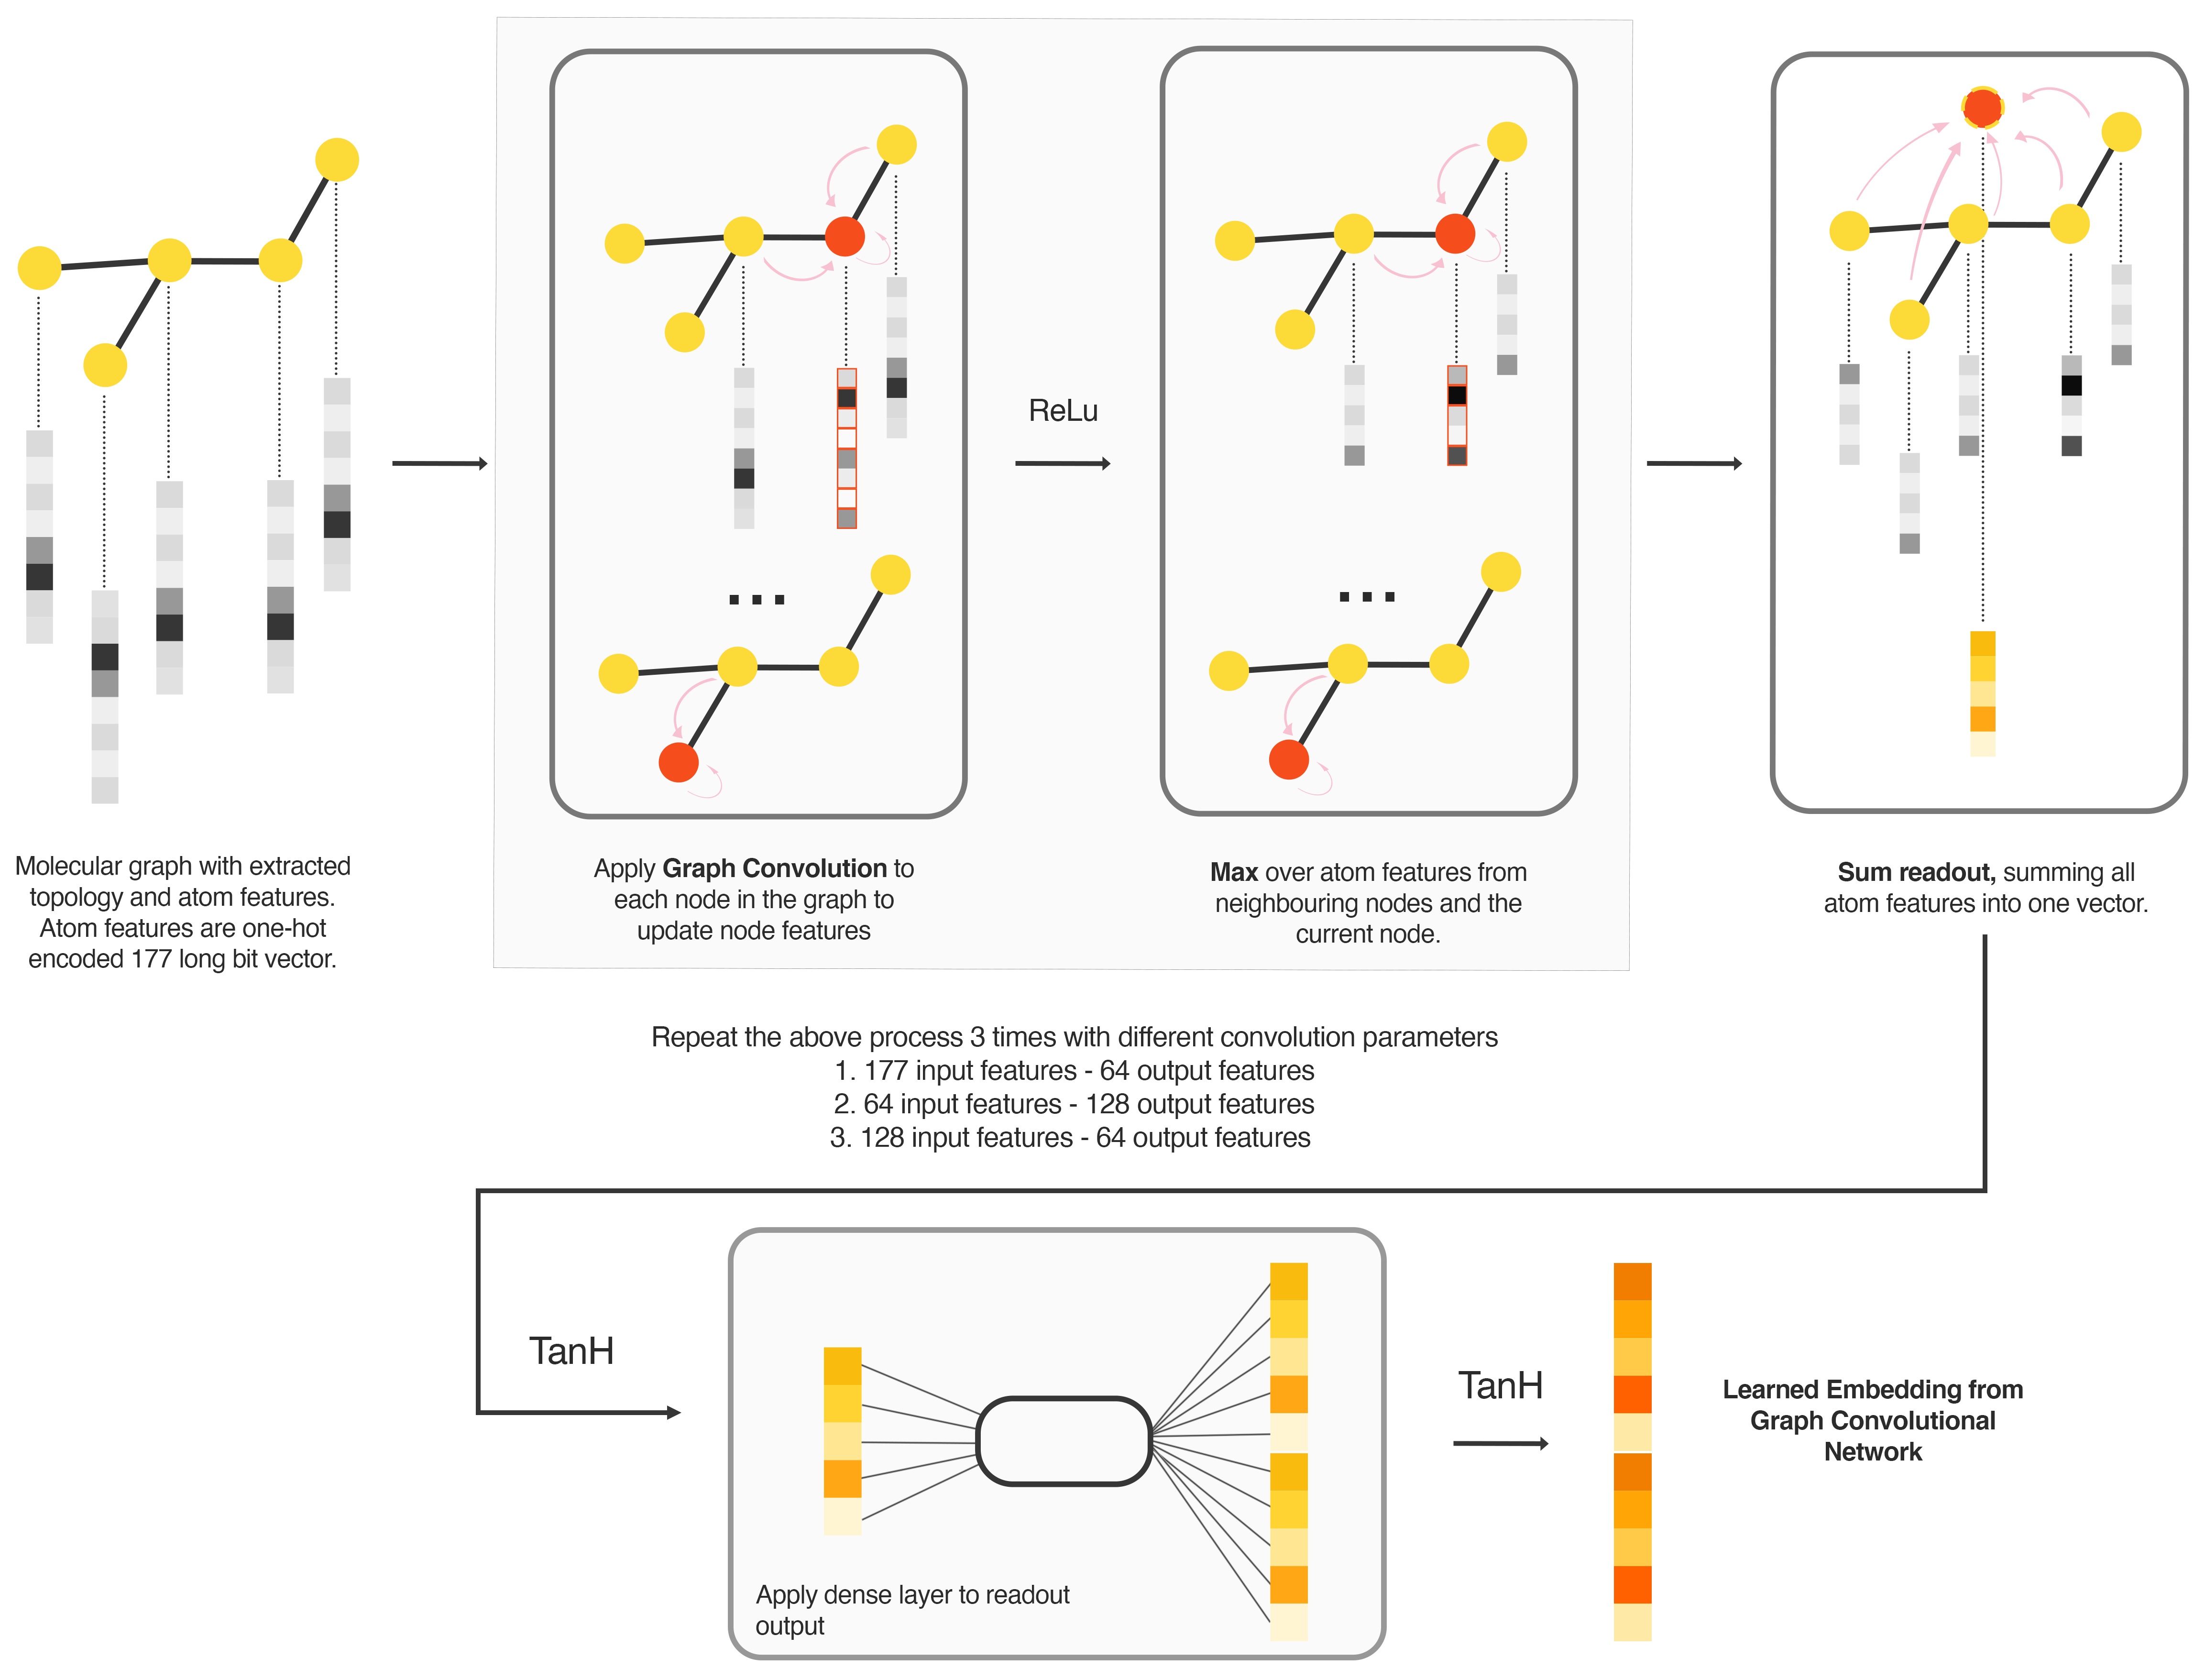
\includegraphics[width=0.75\textwidth]{img/DVGCNArchi.png}
    \caption{Learning an embedding through a Graph Convolutional Network (GCN). The molecule, represented as a graph object with nodes, edges, and atom features, is processed using graph convolutions. A max message-passing function over the current and neighbouring nodes follows each convolution layer. After this process, a sum readout aggregates all atom features into one vector. A tanh function activates this vector, and a dense linear layer processes the output vector. A non-linear tanh function activates this vector to yield the final learned molecular embedding.}
    \label{fig:dvgcnarchi}
\end{figure}

\subsubsection{Graph Convolutional Networks}

Graph convolutional networks (GCNs) are used to learn embeddings for the support and query molecules in latent space. The SMILE molecules are first converted to graph representations and later embedded as vectors in latent space using GCNs and a final dense neural network. Figure~\ref{fig:dvgcnarchi} illustrates the GCN pipeline to learn a molecular embedding. Our study uses the convolutional operator from \citet{kipf2016semi} to process graphs and learn molecular embeddings. We note that back-propagation occurs throughout the whole few-shot learning process, which includes the GCNs. The assays used in testing are unseen during training. However, the molecules used in testing can be encountered during training for different experimental assays. Since they are included in the same dataset (e.g. Tox21 data), these assays are related but not identical.

\begin{equation}
    \label{gcnequation2}
    h_i^{(l+1)} = \sigma(b^{(l)} + \sum_{j\in\mathcal{N}(i)}\frac{1}{c_{ji}}h_j^{(l)}W^{(l)})
\end{equation}

The convolutional layer can be mathematically defined through Equation~\ref{gcnequation2}. $h_j$ is the feature set of the node, $N_i$ is the set of neighbouring nodes $i$, $b$ is the learnable bias, and $c_ji$ is the product of the square root of node degrees. From a message-passing perspective, this can be summarised into the following steps for every node feature space $u$;

\begin{enumerate}
    \item Aggregating the neighbouring representations $h_v$, producing an intermediate representation $\hat{h}_u$.
    \item Transforming $\hat{h}_u$ through a linear projection and a non-linearity function such that $h_u = f(W_u \hat{h}_u)$ \citep{kipf2016semi}.
\end{enumerate}

Three convolutional layers are present in our architecture, after which a maximum function aggregating the node features with the maximum value of the neighbours and the node itself is applied. We highlight that this is not a coarsening operation, as the number of nodes remains the same. Finally, we apply a global pooling layer (readout), in which we sum over the node features of every node in the graph (see Equation~\ref{gcnequationsum}). 

\begin{equation}
    \label{gcnequationsum}
    r^{(i)} = \sum_{k=1}^{N_i} x^{(i)}_k
\end{equation}

A linear transformation is applied to the output from the readout layer, followed by a non-linear activation function, which uses a hyperbolic tangent function (tanh), outputting the final molecule embedding. Table \ref{table:gcn-architecture} contains the architecture utilised for the GCN in this study, and is illustrated in Figure~\ref{fig:dvgcnarchi}.

\begin{table}
    \centering
    \begin{tabular}{@{}lrrl@{}}
    \hline
    \textbf{Layer Type} & \textbf{Input Dimension} & \textbf{Output Dimension} & \textbf{Non-Linearity} \\
    \hline
    GraphConv & 177 & 64 & ReLU \\
    Max Pooling & 64 & 64 & \\
    GraphConv & 64 & 128 & ReLU \\
    Max Pooling & 128 & 128 & \\
    GraphConv & 128 & 64 & ReLU \\
    Max Pooling & 64 & 64 & \\
    SumPool Readout & 64 & 64 & tanh \\
    Linear & 64 & 128 & tanh \\
    \hline  
    \end{tabular}
    \caption{Graph Convolution Network Architecture}
    \label{table:gcn-architecture}
\end{table}

\subsubsection{Benchmark Models}

We use a Random Forest model with 100 decision trees and a Graph Convolutional Network (GCN) to build a baseline to benchmark the purpose-built few-shot learning models. The Random Forest model uses ECFP representations of the molecules of size 2,048 bits for the classification task, using a radius of two. Meanwhile, the same GCN architecture used for the few-shot learning models is used for our benchmark. The designated architecture for the graph convolution network is outlined in Table~\ref{table:benchmarkArchi}. The only addition to the architecture is a final linear, fully-connected layer that takes as input 128 features, which is the size of the embedding used for the experiments to follow. It outputs a feature of size one, onto which we apply a non-linear function, in this case, a Sigmoid function, to output the probabilities for a binary target (${0, 1}$). This binary target signifies whether the molecule belongs to the experimental assay's active or inactive/decoy class. These two models are trained on a small support set, sampled from the targets assigned for testing. The remaining molecules that are not utilised for training are used to predict the respective class.

We also perform a final benchmark test in retrospect by taking a random selection of query molecules from a test target, generating the ECFP with the same parameters as mentioned earlier and then calculating the Tanimoto distance to classify the remaining test molecules based on this distance. However, we find that this does not hold any significant predictive capability. 

\begin{table}
    \centering
    \begin{tabular}{@{}lrrl@{}}
    \hline
    \textbf{Layer} & \textbf{Input Dimension} & \textbf{Output Dimension} & \textbf{Non-Linearity} \\
    \hline
    GraphConv   & 177   & 64    & Relu \\
    Max Pooling & 64    & 64    &  \\
    GraphConv   & 64    & 128   & Relu \\
    Max Pooling & 64    & 64    &  \\
    GraphConv   & 128   & 64    & Relu \\
    Max Pooling & 64    & 64    &  \\
    Sum Pooling & 64    & 64    & TanH \\
    Linear      & 64    & 128   & TanH \\
    Linear      & 128   & 1     & Sigmoid \\
    \hline
    \end{tabular}
    \caption{Benchmark Neural Network for Few-Shot Learning}
    \label{table:benchmarkArchi}
\end{table}

\subsubsection{Few-Shot Learning Models}

The generated molecular embeddings from the GCN are used as inputs for the few-shot learning architectures. The models discussed in this section, excluding the benchmark model, use the embeddings generated from the GCN, grouped in support and query sets, to learn the kernel function. These models include Siamese Networks, Matching Networks, Prototypical Networks and Relation Networks. Table \ref{table:relation-neural-net} tabulates the network used to generate the relation score in the Relation Networks architecture. The GCN architecture remains unchanged in all experiments to compare the model's effectiveness objectively. Figure~\ref{fig:schematic-training} illustrates the rationale behind few-shot machine learning for this problem domain. The molecules used in training and testing can be shared; however, the target information imparting activity in a specific experimental assay must be different. This separation entails that we present the machine learning model with information from previously unseen experimental assays during testing. For example, training can be done on molecular activity for nuclear receptor assays in Tox21 and then tested on the remaining assays, which would have never been seen during training.

\begin{figure}[ht!]
    \centering
    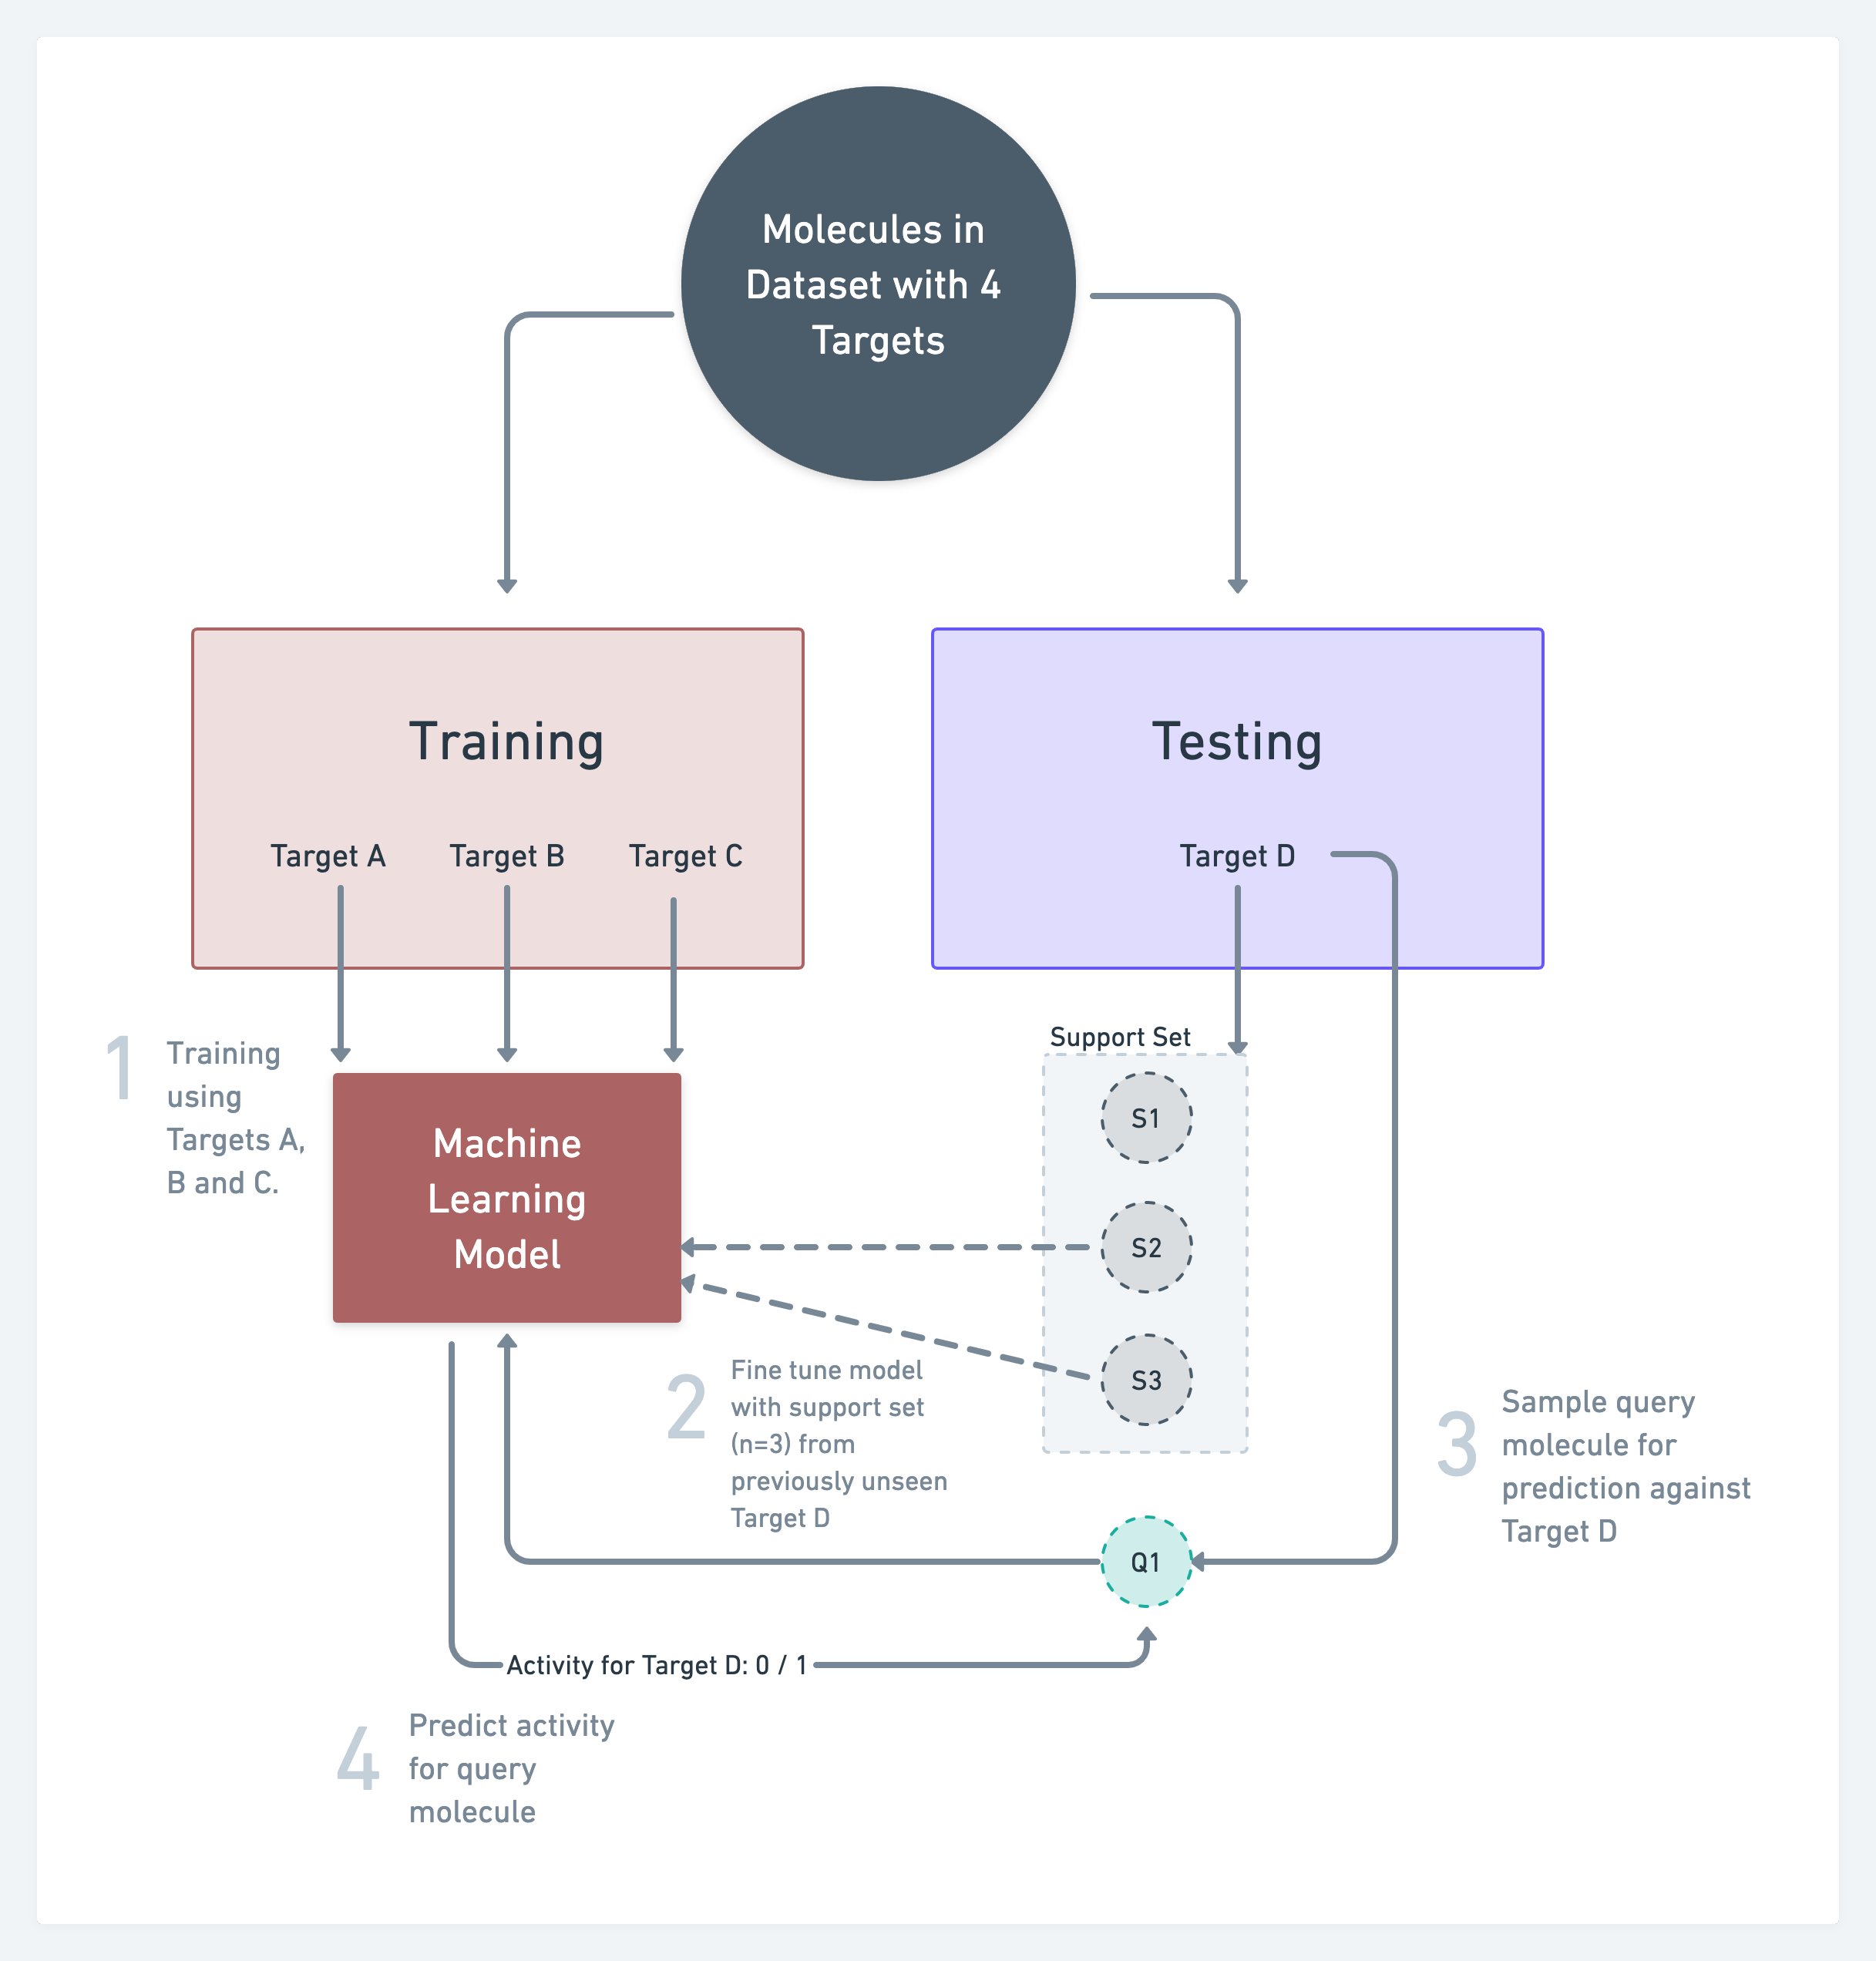
\includegraphics[width=0.75\textwidth]{img/Schematic Training.png}
    \caption{Schematic illustrating how the few-shot learning machine learning on a molecular dataset works. The same molecules can be used during training and testing; however, these molecules would impart different information based on the target or experimental assay. The targets used in testing are previously unseen, except for the few molecules sampled in the support set (S\textsubscript{1-3}), which are used to fine-tune the ML model and impart some information about Target D. Query molecule Q\textsubscript{1} is sampled from Target D to be predicted using the ML model.}
    \label{fig:schematic-training}
\end{figure}

\begin{table*}[h]
    \centering
    \begin{tabular}{@{}lrrl@{}}
    \hline
    Layer Type & Input Dimension & Output Dimension & Non-Linearity \\
    \hline
    Linear  & 256   & 128   & ReLU \\
    Linear  & 128   & 64    & ReLU \\
    Linear  & 64    & 8     & ReLU \\
    Linear  & 8     & 2     & Sigmoid \\
    \hline
    \end{tabular}
    \caption{The architecture for generating the relation score using function $g_\theta$.}
    \label{table:relation-neural-net}
\end{table*}

We reproduce the work of \citet{altae2017low} from scratch and apply the IterRefLSTM to the embeddings in all architectures to effectively compare our contribution to past work. Additionally, we also provide implementations for the Prototypical Networks and Relation Networks. All the experiments are run on Google Colaboratory, and all implementations are open-sourced on GitHub\footnote{Accessed From: \url{https://github.com/danielvlla/Few-Shot-Learning-for-Low-Data-Drug-Discovery}}. As emphasised by \citet{vinyals2016matching} and \citet{snell2017prototypical}, training and testing conditions should match during few-shot learning. Therefore, the same support set composition used to train the model is used during test time. For example, if we train using 10-shot learning, testing is carried out with 10-shot support sets. We remind the reader that testing is carried out on a new, previously unseen target. After the support set has been sampled, the rest of the data for the target being tested is used as query data. This process is repeated 20 times, and the mean and standard deviation of the ROC-AUC and PR-AUC scores from these 20 rounds are reported as the final classification result.

\subsubsection{Evaluation}

The evaluation metrics we use are the Area Under Curve (AUC) of the Receiver Operating Characteristic (ROC) curve and the Precision-Recall Curve (PR-AUC). To determine our classifier's predictive power, we use the ROC Area Under Curve (AUC) (ROC-AUC) as this affords a more nuanced approach than the accuracy metric, providing visibility into thresholds one can utilise to ameliorate predictions. \citet{altae2017low} also report ROC-AUC results; however, we believe this metric alone does not adequately measure the performance of the machine learning models due to the highly imbalanced nature of the data at hand. In virtual screening, detecting rare events (equivalent to our minority active class) holds significant importance, as active compounds against a specific target should be identified from the compound database. However, we do not disregard the importance of correct classification of the majority inactive/decoy class, as this is also important for filtering out thousands of screened compounds. As the active class is the minority class, PR-AUC is used to evaluate how well the model can classify the active class.

We apply statistical analysis to the ROC-AUC and PR-AUC scores from the 20 test rounds for each experiment to establish whether there are significant differences between the few-shot learning models. The scores are compared against the scores from the model that obtained the best result for the same conditions. Comparison of results between two models is carried out using the Mann-Whitney U-test, also referred to as the Wilcoxon rank sum test \citep{mann1947test}.

\section{Implementation Details}

The machine learning models were developed using Python 3.7. Most packages were installed using Pip 21.0.1; however, Conda 4.10.3 was also used to install packages not found on the Python Package Index (PyPi)\footnote{Accessed from: \url{https://pypi.org/}. Last Accessed: 26/05/2022}. Pip and conda are package management systems for Python, allowing users to install and run packages and their dependencies conveniently. The specific versions of each toolkit are specified in Table~\ref{tab:versions}.

\begin{table}
    \centering
    \begin{tabular}{@{}lll@{}}
        \hline
        \textbf{Package} & \textbf{Version} & \textbf{Description} \\
        \hline
        PyTorch & 1.9.0 & Machine learning framework \\
        Scikit-Learn & 1.0.1 & Machine Learning Library \\
        Deep Graph Library (DGL) & 0.7.2 & Deep learning on graphs \\
        DGL-LifeSci & 0.2.8 & Cheminformatics graph functions \\
        RDKit & 2021.09.2 & Cheminformatics Toolkit \\
        DeepChem & 2.6.0.dev & Cheminformatics Machine Learning \\
        Pandas & 1.1.5 & Data manipulation and preparation \\
        Numpy & 1.19.5 & Adds support for multi-dimensional arrays \\
        ChemBL Structure Pipeline & 1.0.0 & Used to standardise molecules \\
        NetworkX & 2.6.3 & Used to visualise graphs \\
        TQDM & 4.59 & Progress bars library \\
        SciPy & 1.7.1 & Statistical Analysis \\
        \hline
    \end{tabular}
    \caption{Python libraries utilised for this project.}
    \label{tab:versions}
\end{table}

All the experiments were run on Google Colaboratory\footnote{Accessed from: \url{https://colab.research.google.com/}. Last Accessed: 26/05/2022}, Colab in short, and this platform's details are specified in Table~\ref{tab:hardware}.

\begin{table}
    \centering
    \begin{tabular}{@{}lll@{}}
        \hline
        \textbf{Type} & \textbf{Model} & \textbf{Details} \\
        \hline
        CPU & Intel (R) Xeon & 2.20~Ghz 4 Cores \\
        GPU & Nvidia Tesla P100 & 16~GB using Cuda 11.1 \\
        RAM & N/A & 25~GB \\
        \hline
    \end{tabular}
    \caption{Hardware provisioned in Google Colab.}
    \label{tab:hardware}
\end{table}
